\documentclass[compress,blue]{beamer}
\usepackage{etex}
\mode<presentation>

\usetheme{Copenhagen}
% other themes: AnnArbor, Antibes, Bergen, Berkeley, Berlin, Boadilla, boxes, CambridgeUS, Copenhagen, Darmstadt, default, Dresden, Frankfurt, Goettingen, Warsaw
% Hannover, Ilmenau, JuanLesPins, Luebeck, Madrid, Maloe, Marburg, Montpellier, PaloAlto, Pittsburg, Rochester, Singapore, Szeged, classic

%\usecolortheme{lily}
% color themes: albatross, beaver, beetle, crane, default, dolphin, dov, fly, lily, orchid, rose, seagull, seahorse, sidebartab, structure, whale, wolverine

%\usefonttheme{serif}
% font themes: default, professionalfonts, serif, structurebold, structureitalicserif, structuresmallcapsserif

% pdf is displayed in full screen mode automatically
%\hypersetup{pdfpagemode=FullScreen}

% define your own colours:
\definecolor{Red}{rgb}{1,0,0}
\definecolor{Blue}{rgb}{0,0,1}
\definecolor{Green}{rgb}{0,1,0}
\definecolor{magenta}{rgb}{1,0,.6}
\definecolor{lightblue}{rgb}{0,.5,1}
\definecolor{lightpurple}{rgb}{.6,.4,1}
\definecolor{gold}{rgb}{.6,.5,0}
\definecolor{orange}{rgb}{1,0.4,0}
\definecolor{hotpink}{rgb}{1,0,0.5}
\definecolor{newcolor2}{rgb}{.5,.3,.5}
\definecolor{newcolor}{rgb}{0,.3,1}
\definecolor{newcolor3}{rgb}{1,0,.35}
\definecolor{darkgreen1}{rgb}{0, .35, 0}
\definecolor{darkgreen}{rgb}{0, .6, 0}
\definecolor{darkred}{rgb}{.75,0,0}

\xdefinecolor{olive}{cmyk}{0.64,0,0.95,0.4}
\xdefinecolor{purpleish}{cmyk}{0.75,0.75,0,0}

% \usepackage{beamerinnertheme_______}
% inner themes include circles, default, inmargin, rectangles, rounded

%\usepackage{beamerouterthemesmoothbars}
% outer themes include default, infolines, miniframes, shadow, sidebar, smoothbars, smoothtree, split, tree

\useoutertheme[subsection=false]{smoothbars}

% to have the same footer on all slides
%\setbeamertemplate{footline}[text line]{xxx xxx xxx}
%\setbeamertemplate{footline}[text line]{} % or empty footer

% include packages
\usepackage{amsmath}
\usepackage{epsfig}
\usepackage{graphicx}
\usepackage[all,knot]{xy}
\xyoption{arc}
\usepackage{multimedia}
\usepackage{hyperref}
\usepackage{setspace}
\usepackage{tikz}
\usetikzlibrary{positioning}

\usepackage{animate}


\title{The Adaptive Method of Lines}
\subtitle{CDEs Group Presentation}
\author{Shian Su, Ria Szeredi and Kenneth Young}
\institute{University of Melbourne}
\date{$23^{\text{rd}}$ of May, 2016}

\begin{document}

\frame{\titlepage}

\section[Outline]{}
\frame{\tableofcontents}

\section{Introduction}

\subsection{Standard method of lines}
\frame{\frametitle{Motivation}
\textbf{Method of lines}
\vspace{0.25cm}
\begin{itemize}
    \item Discretise in space (eg. using finite difference) to generate a system of ODEs.
    \vspace{0.25cm}
    \item Solve the system using some solver such as ode15s.
    \vspace{0.25cm}
    \item Temporal accuracy handled by the ODE solver, however spatial accuracy results from the discretisation used.
\end{itemize}
}

\subsection{Motivation}
\frame{\frametitle{Motivation}
\textbf{Problems with Uniform Mesh}
\vspace{0.25cm}
\begin{itemize}
    \item Method of lines discretises the space uniformly.
    \vspace{0.25cm}
    \item What if our problem has \emph{steep fronts}?
        \vspace{0.25cm}
        \begin{itemize}
            \item[--] Low density uniform mesh doesn't approximate steep fronts well.
            \vspace{0.25cm}
            \item[--] High density uniform mesh achieves high spatial accuracy, but wastes nodes in regions of low activity.
        \end{itemize}
\end{itemize}
}

\subsection{Method of lines used to solve Burgers' equation}
\frame{\frametitle{Method of Lines - Burgers' Equation}
\begin{itemize}
	\item Bad approximation in regions of high spatial activity when grid is uniform. Here we use 201 nodes.
\end{itemize}
\animategraphics[controls, width=1\linewidth]{1}{images/MoL_burgers_}{0}{10}
}

\section{Adaptive Method of Lines}
\subsection{Mesh Adaptation}
\frame{\frametitle{Mesh Adaptation}
\begin{itemize}
	\item Want to adapt the spatial mesh such that nodes are efficiently placed.
	\begin{itemize}
		\item[--] Static moving mesh.
		\item[--] Static grid refinement.
		\item[--] Dynamic mesh.
	\end{itemize}
\end{itemize}
}


\subsection{Equidistribution principle}
\frame{\frametitle{Equidistribution Principle}
\textbf{Tracking the action}
\begin{itemize}
    \item Want to assign more nodes to areas with high activity.
    \item Use some monitor function $m(x)$ to measure the activity in a region.
    \item Choose the $x_i$ such that for all $i$,\\ $\int\limits_{x_{i-1}}^{x^{i}} m(x) \, \text{d}x = \int\limits_{x_{i}}^{x^{i+1}} m(x) \, \text{d}x$ (equidistribution).
    \item In practice equidistribution is considered optimal, but some suboptimal methods may be used to have roughly equal distribution in order to reduce computational effort.
\end{itemize}
}

\subsection{Choice of monitor function}
\frame{\frametitle{Choice of Monitor Function}
\begin{itemize}
    \item Arc length $m(x) = \sqrt{\alpha + u_x^2(x)}$.
    \vspace{0.25cm}
    \item Local curvature $m(x) = |u_{xx}(x)|$.
    \vspace{0.25cm}
    \item Other options involving many tuning parameters exist.
    \vspace{0.25cm}
    \item Since the true solution is not known, derivatives must be estimated. Can use natural splines to interpolate current solution and use its derivatives as approximation.
\end{itemize}
}

\frame{\frametitle{Uniform vs Equidistributed Arclengths (n=21)}
\centering 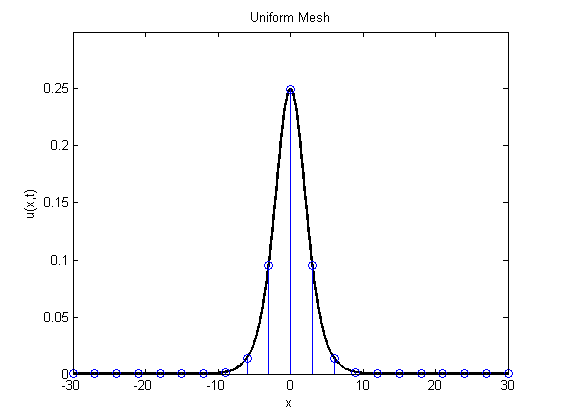
\includegraphics[scale=.35]{images/mesh_uniform.png} 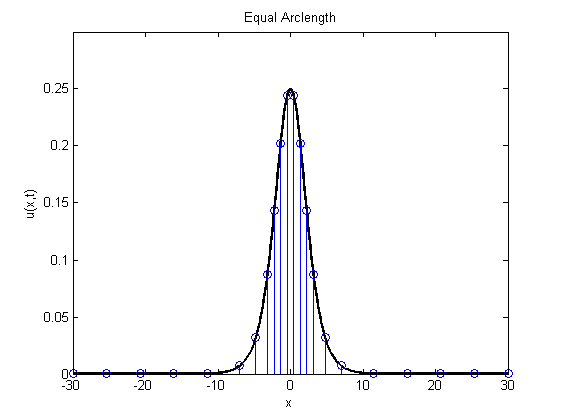
\includegraphics[scale=.35]{images/mesh_arclength.png}
}

\section*{}
\frame{\frametitle{Example Problems}
\begin{itemize}
    \item Burgers' Equation \\
    $u_{t} + u u_{x} + u_{xx} = 0$
    \vspace{0.4cm}
    \item Korteweg-de Vries (KDV) Equation \\
    $u_{t} + u_{xxx} + 6u u_{x} = 0$
    \vspace{0.25cm}
\end{itemize}
}

\section{Static Method}
\subsection{Moving Mesh theory and examples}
\frame{\frametitle{Moving Mesh}
\begin{itemize}
    \item Fix the number of nodes.
    \vspace{0.25cm}
    \item Pause the PDE solver at a set interval to move the mesh nodes to achieve equidistribution.
    \vspace{0.25cm}
    \item Interpolate the solution from old mesh to generate initial conditions for new mesh.
\end{itemize}
}

\frame{\frametitle{Moving Mesh - KDV Equation Example 1}
\begin{tabular}{c|c|c}
	\hline
	\rule{0pt}{2ex} Mesh Adaptions & \# of Mesh Nodes & Computation Time \\
	\hline
	\rule{0pt}{2ex} 10 & 151 & 8.9 sec \\
\end{tabular}
\animategraphics[controls, width=1\linewidth]{1}{images/static_moving_KDV_dt10_}{0}{10}
}

\frame{\frametitle{Moving Mesh - KDV Equation Example 1 Error}
\centering 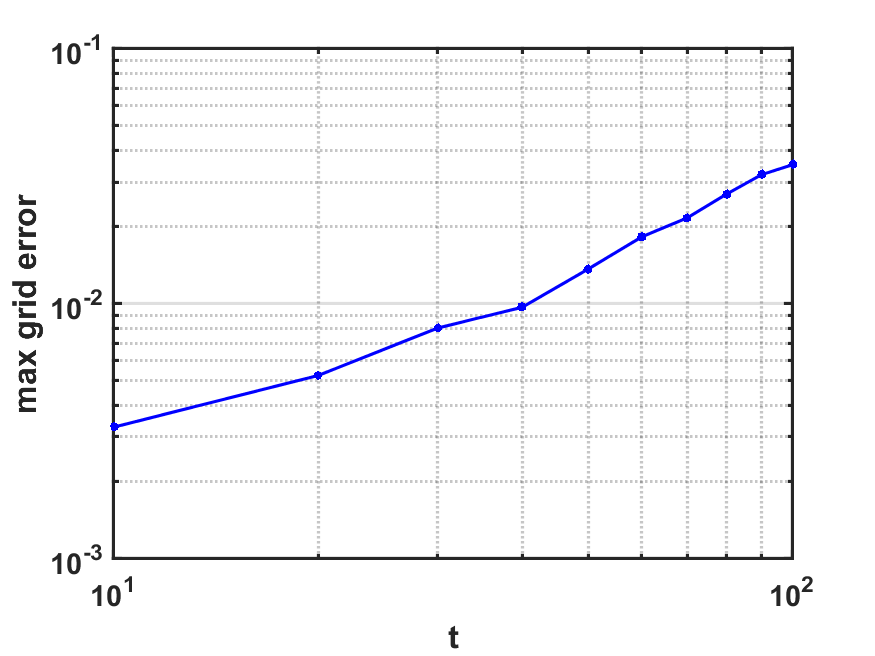
\includegraphics[height=0.8\textheight]{images/static_moving_KDV_error_dt10.png}
}

\frame{\frametitle{Moving Mesh - KDV Equation Example 2}
\begin{tabular}{c|c|c}
	\hline
	\rule{0pt}{2ex} Mesh Adaptions & \# of Mesh Nodes & Computation Time \\
	\hline
	\rule{0pt}{2ex} 50 & 151 & 19.6 sec \\
\end{tabular}
\animategraphics[controls, width=1\linewidth]{5}{images/static_moving_KDV_dt2_}{0}{50}
}

\frame{\frametitle{Moving Mesh - KDV Equation Example 2 Error}
\centering 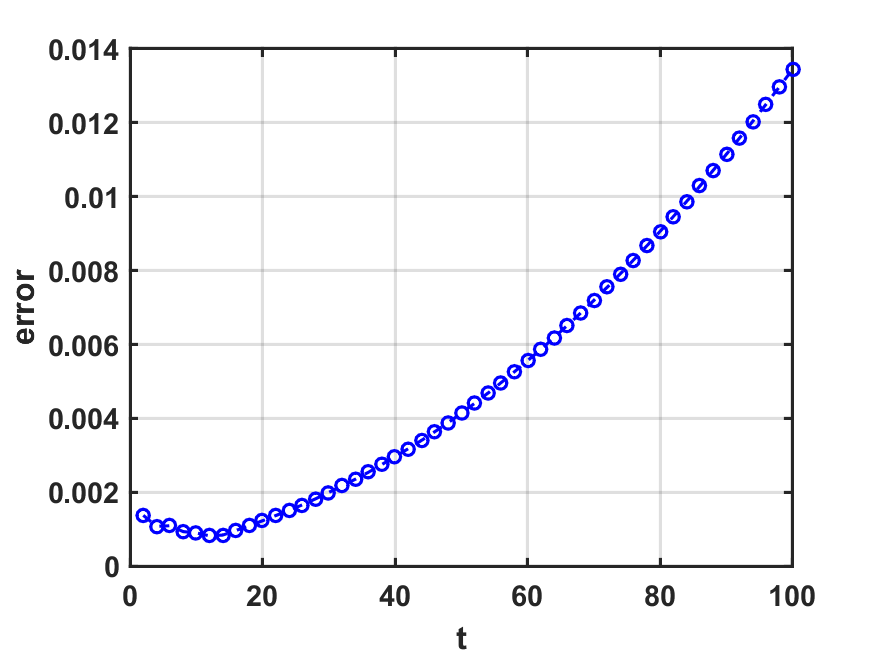
\includegraphics[height=0.8\textheight]{images/static_moving_KDV_error_dt2.png}
}

\frame{\frametitle{Moving Mesh - Burgers' Equation Example 1}
\begin{tabular}{c|c|c}
	\hline
	\rule{0pt}{2ex} Mesh Adaptions & \# of Mesh Nodes & Computation Time \\
	\hline
	\rule{0pt}{2ex} 10 & 375 & 5.8 sec \\
\end{tabular}
\animategraphics[controls, width=1\linewidth]{1}{images/static_moving_burgers_dt01_}{0}{10}
}

\frame{\frametitle{Moving Mesh - Burgers' Equation Example 1 Error}
\centering 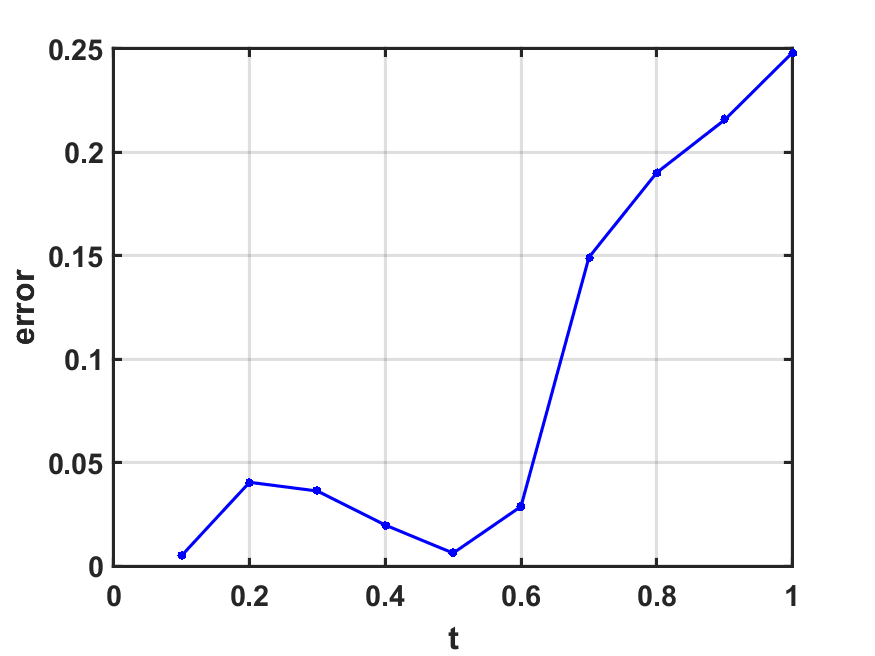
\includegraphics[height=0.8\textheight]{images/static_moving_burgers_error_dt01.png}
}

\frame{\frametitle{Moving Mesh - Burgers' Equation Example 2}
\begin{tabular}{c|c|c}
	\hline
	\rule{0pt}{2ex} Mesh Adaptions & \# of Mesh Nodes & Computation Time \\
	\hline
	\rule{0pt}{2ex} 100 & 251 & 36.1 sec \\
\end{tabular}
\animategraphics[controls, width=1\linewidth]{10}{images/static_moving_burgers_dt001_}{0}{100}
}

\frame{\frametitle{Moving Mesh - Burgers' Equation Example 2 Error}
\centering 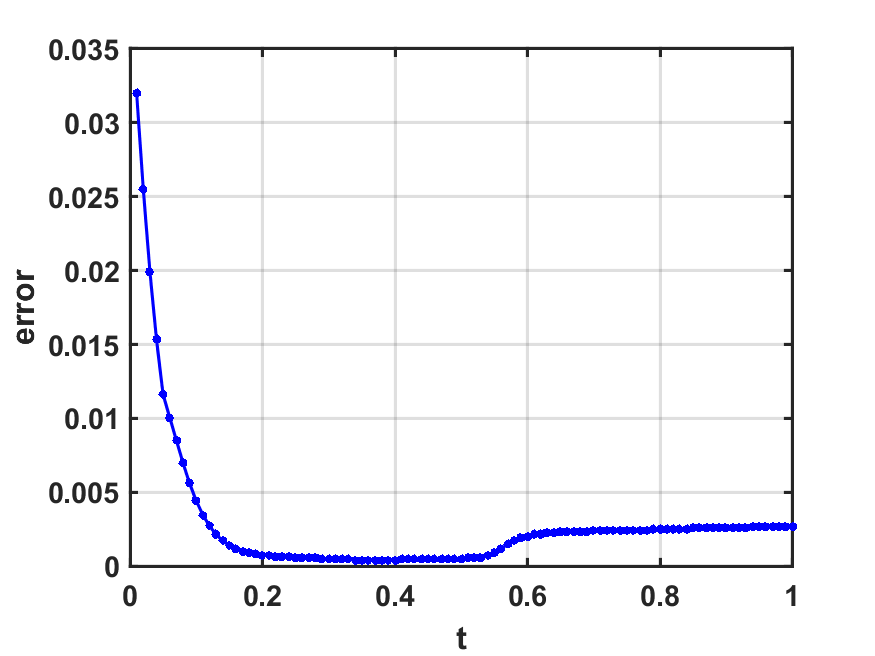
\includegraphics[height=0.8\textheight]{images/static_moving_burgers_error_dt001.png}
}

%\subsection{Mesh Refinement theory and examples}
%\frame{\frametitle{Mesh Refinement}
%\begin{itemize}
%\item Just as in moving mesh, the mesh is updated at set intervals.
%\vspace{0.25cm}
%\item Rather than trying to achieve equidistribution, A uniform grid is used as a skeleton, at each pause the monitor function is measured between each node, additional nodes with uniform spacing is added in between nodes that exceed some threshold.
%\vspace{0.25cm}
%\item Interpolate and continue.
%\end{itemize}
%}

\subsection{Mesh Refinement theory and examples}
\frame{\frametitle{Mesh Refinement}
\begin{itemize}
	\item Just as in moving mesh, the mesh is updated at set intervals.
	\vspace{0.25cm}
	\item Procedure for each mesh adaption:
         \setbeamertemplate{enumerate items}[default]
		\begin{enumerate}
			\item Reset to uniform base grid.
			\item Evaluate monitor function between each pair of nodes.
			\item If threshold exceeded, add nodes with uniform spacing
			\item If below threshold, remove some nodes.
			\item Interpolate and repeat.
		\end{enumerate}
	\vspace{0.25cm}
\end{itemize}
\vspace{0.25cm}
\begin{center}
	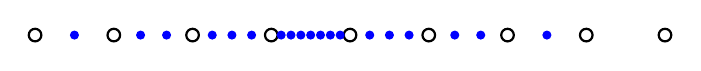
\begin{tikzpicture}
		\uncover<2->{
		\foreach \x in  {-4,-3,-2,-1,0,1,2,3,4} 
		\draw [thick] (\x,0) circle [radius=0.08];}
		\uncover<3->{
		\draw [fill,color=Blue] (-3.5,0) circle [radius=0.05];
		\foreach \x in  {-2.66,-2.33} 
		\draw [fill,color=Blue] (\x,0) circle [radius=0.05];
		\foreach \x in  {-1.75,-1.5,-1.25} 
		\draw [fill,color=Blue] (\x,0) circle [radius=0.05];
		\foreach \x in  {-0.875,-0.75,-0.625,-0.5,-0.375,-0.25,-0.125} 
		\draw [fill,color=Blue] (\x,0) circle [radius=0.05];
		\foreach \x in  {0.25,0.5,0.75} 
		\draw [fill,color=Blue] (\x,0) circle [radius=0.05];
		\foreach \x in  {1.33,1.66} 
		\draw [fill,color=Blue] (\x,0) circle [radius=0.05];
		\draw [fill,color=Blue] (2.5,0) circle [radius=0.05];}
	\end{tikzpicture}
\end{center}
}

\frame{\frametitle{Mesh Refinement - Burgers' Equation Example 1}
\begin{tabular}{c|c|c}
	\hline
	\rule{0pt}{2ex} Mesh Adaptions & \# of Mesh Nodes & Computation Time \\
	\hline
	\rule{0pt}{2ex} 10 & $\approx$ 268.5 & 6.0 sec \\
\end{tabular}
\animategraphics[controls, width=1\linewidth]{1}{images/static_adapt_burgers_dt01_}{0}{10}
}

\frame{\frametitle{Mesh Refinement - Burgers' Equation Example 1 Error}
\centering 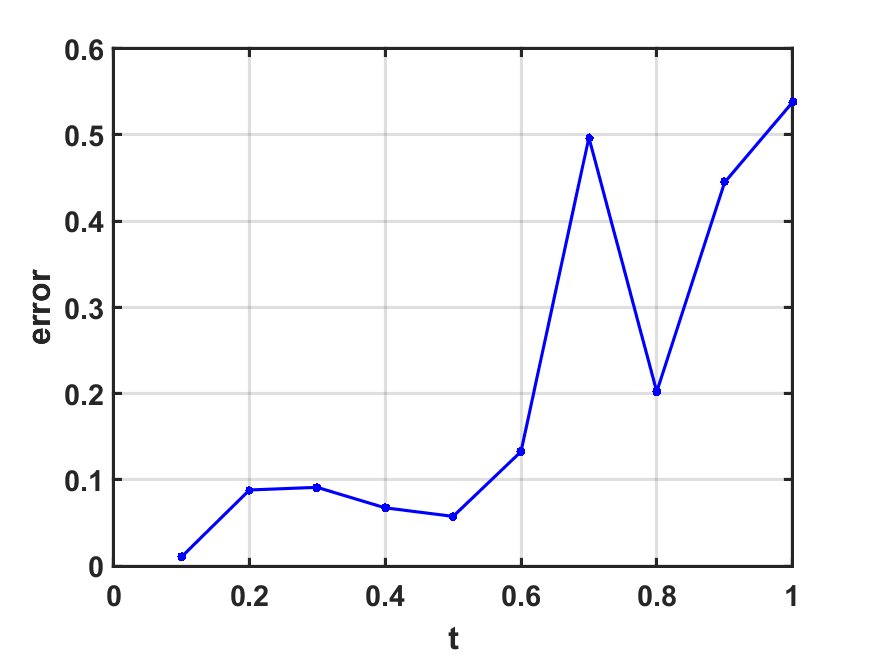
\includegraphics[height=0.8\textheight]{images/static_adapt_burgers_error_dt01.png}
}

\frame{\frametitle{Mesh Refinement - Burgers' Equation Example 2}
\begin{tabular}{c|c|c}
	\hline
	\rule{0pt}{2ex} Mesh Adaption & \# of Mesh Nodes & Computation Time \\
	\hline
	\rule{0pt}{2ex} 100 & $\approx$ 152.5 & 41.2 sec \\
\end{tabular}
\animategraphics[controls, width=1\linewidth]{10}{images/static_adapt_burgers_dt001_}{0}{100}
}


\frame{\frametitle{Mesh Refinement - Burgers' Equation Example 2 Error}
\centering 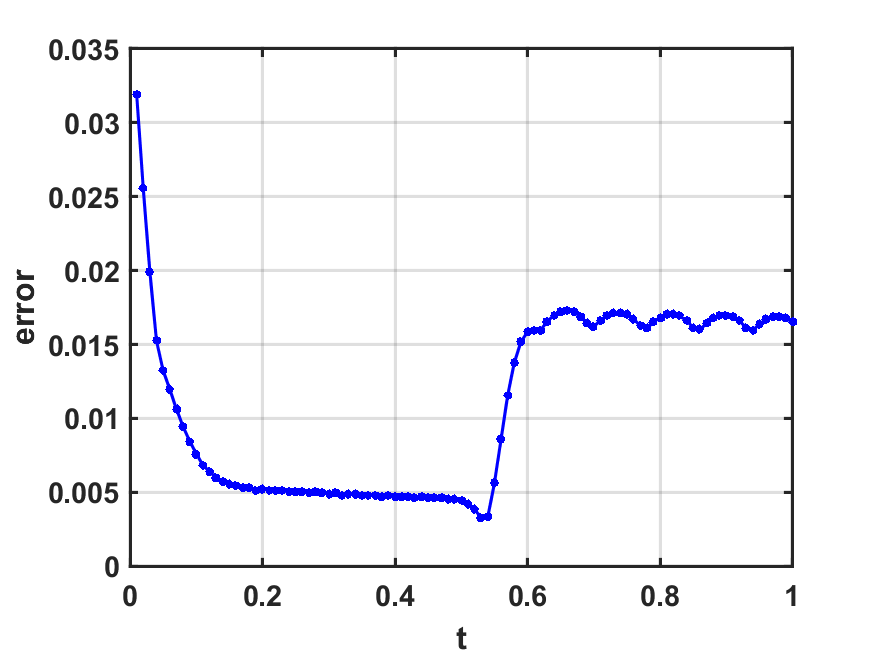
\includegraphics[height=0.8\textheight]{images/static_adapt_burgers_error_dt001.png}
}

\section{Dynamic Method}
%\subsection{Dynamic Method}
\frame{\frametitle{Problems with Static Grid Refinement}
\begin{itemize}
	\item Infrequent grid refinement can cause the mesh to lag behind the moving solution.
	\vspace{0.25cm}
	\item Refining too often is computationally expensive and negates any benefits from adaptive mesh.
	\vspace{0.25cm}
	\item In dynamic refinement methods, positions of nodes are functions of time.
	\vspace{0.25cm}
\end{itemize}
}

\frame{\frametitle{Dynamic Method}
\begin{itemize}
	\item May be possible to use a priori information to generate functions for the wave to travel along. For example the characteristic curves along which the solution is constant. For a simple moving wave this tracks positions on the wave-front.
	\vspace{0.25cm}
	\item Requires specific a priori knowledge of the problem, not always possible to derive characteristic curves.
\end{itemize}
}

\frame{\frametitle{Dynamic Method - Burgers' Equation Example}
\begin{tabular}{c|c|c}
	\hline
	\rule{0pt}{2ex} Mesh Adaptions & \# of Mesh Points & Computation Time \\
	\hline
	\rule{0pt}{2ex} 10 & 51 & 15.4 sec \\
\end{tabular}
\animategraphics[controls, width=1\linewidth]{1}{images/dynam_burgers_}{1}{11}
}

\section*{}
\frame{\frametitle{Summary}
\begin{itemize}
	\item Problems arise when uniform grid used in Method of Lines.
	\vspace{0.25cm}
	\item Solution: adapt the grid to account for regions of high activity.
	\vspace{0.25cm}
	\item Static adaptation: refine the grid at discrete time steps.
	\vspace{0.25cm}
	\item Dynamic adaptation: positions of nodes are functions of time.
\end{itemize}
}

\begin{frame}%[allowframebreaks]
        \frametitle{References}
        \begin{itemize}
        		\item Vande Wouwer, Saucez and Schiesser, \emph{The Adaptive Method of Lines}, Chapman and Hall, 2001.
		\item Vande Wouwer, Saucez and Schiesser, \emph{Simulation of ODE/PDE Models with MATLAB, OCTAVE and SCILAB}, Springer 2014.
		\item Marlow, \emph{Moving Mesh Methods for Solving Parabolic Partial Differential Equations}, Ph. D. Thesis, 2010.
	\end{itemize}
%        \bibliographystyle{amsalpha}
%        \nocite{*}
%        \bibliography{refs}
\end{frame}


\frame{
    \begin{center}
        \huge
        This is the last slide.\\
        \vspace{1cm}
        Any questions?
    \end{center}
}

\end{document} 